\chapter{Ontwikkeling cross platforme mobiele applicatie}
\label{ch:ontwikkelingcrossplatformapp}
\section{Analyse van het project}
Als start van het project werd er een analyse gemaakt van de co-promotor
een analyse gemaakt van de functionele requirements.

De analyse bestaat uit het sturen van een query naar de databank die draait in een webservice.
Op deze manier worden de gegevens omgezet naar JSON \footnote{JavaScript Object Notation}, een gegevensformaat dat makkelijk
leesbaar is voor toepassingen en vaak gebruikt wordt in webservice.  Het grote voordeel van \cite{inleidingtotjson}
is dat het makkelijk leesbaar/te genereren is voor/door toepassingen.

\section{Ontwikkeling van de ASP.NET MVC Web api}
De ASP.NET MVC Web api heeft in deze toepassing 2 functies. Enerzijds wordt de web api gebruikt om gebruikers zich te laten
authenticeren bij het Active Directory domein van de Gentse Politie, anderzijds levert de web api de gegevens die binnen
de applicatie nodig zijn voor de gebruikers. Deze authenticatie gebeurt aan de hand van tokens die een bepaalde tijd geldig zijn
(in deze casus een week). Nadien moet de gebruiker zich opnieuw authenticeren aan de hand van de inloggegevens. Dit om opnieuw een
token met geldigheid van 1 week te verkrijgen. De tokens zijn verplicht toe te voegen aan de request. In dit niet gebeurt stuurt
de server een antwoord dat men geen toegang heeft tot de aangevraagde resources. De schematische voorstelling van deze techniek,
kan u terugvinden op de volgende pagina.

\begin{figure}[ht!]
\centering
\caption{Token-authenticatie met ASP.NET MVC Web api}
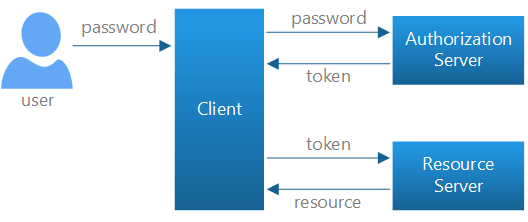
\includegraphics[width=90mm]{./img/authentication.png}
\end{figure}

\section{Ontwikkeling van de cross platforme mobiele applicatie}
\subsection{Gedeelde code}
Om de applicaties op een zo efficiënte manier te ontwikkelen, wordt er code gedeeld tussen de deelprojecten van de 3 mobiele
platformen. Concreet houdt dit in de code die nodig is voor het ophalen van de gegevens uit de webservice gemeenschappelijk
gesteld wordt voor zowel het Android-, als het iOS- en Windowsphone-project. Ook het domeinmodel wordt gemeenschappelijk
gedefinieërd voor de drie mobiele applicaties.

\subsubsection{Code om data op te halen uit de REST-api}

%% Opdelen in kleinere stukken en deze kleine stukken uitleggen

De code die absolute gedeeld word wegens efficientieredenen is de code om de data op te halen uit de REST-service.
Hieronder vindt u het voorbeeld dat als basis diende voor de ontwikkeling van de cross platforme mobiele applicatie.
De volledige code met uitgebereide stappen om dit voorbeeld te ontwikkelen is beschikbaar op \citep{buildappwithnativeuiusingxamarininvisualstudio}.

Ter voorbereiding van de logica om data uit een REST-api op te halen hebben we een klasse nodig die de entiteit uit het
domein van de toepassing voorziet. In dit geval gaat het om de klasse Persoon met onder andere de velden Voornaam, Familienaam, Geslacht.
\begin{lstlisting}
namespace MobileApp
{
  public class Persoon
  {
    public string Voornaam {get; set;}
    public string Familienaam {get; set;}
    public string Geslacht{get; set;}
  }
}
\end{lstlisting}
Nu de deze domeinklasse gedefinieërd is, kunnen we verdergaan met een klasse aan te maken voor het effictief ophalen van
gegevens uit de REST-service. Hierbij is het belangrijk om op te merken dat deze code asynchroon op de main-thread van de
applicatie word uitgevoerd. Voorlopig ziet de klasse er als volgt uit:
\begin{lstlisting}
using System.Threading.Tasks;
using Newtonsoft.Json;
using System.Net.Http;
namespace MobileApp
{
  public class DataService
  {
    public async Task<string> getData(string queryString)
    {
      // Implementatie DataService.getData(string queryString)
    }
  }
}
\end{lstlisting}
Nu we de methode gedefinieërd hebben, kunnen we deze verder implementeren.
Deze implementatie zal bestaan uit 2 delen. Enerzijds zal de data opgehaald uit de REST-api, anderzijds zal de opgehaald data
omgevormd worden tot objecten van het type "Persoon". Dit type is hierboven reeds gedefinieërd.

De volgende code die we toevoegen aan de klasse "DataService", is de code om de data als JSON binnen te halen.
Hiervoor moet er eerst een instantie van de klasse HttpClient (uit de namespace System.Net.Http) aangemaakt worden.
\begin{lstlisting}

// import statements

      // Implementatie DataService.getData(string queryString)
      // een instantie van de klasse HttpClient aanmaken
      HttpClient client = new HttpClient();

\end{lstlisting}
Nu de instantie van HttpClient geinstanceerd is, kan deze gebruikt worden om data op te halen bij de webservice.
Het ophalen van de data gebeurt aan de hand van onderstaande code:
\begin{lstlisting}
  using System.Threading.Tasks;
  using Newtonsoft.Json;
  using System.Net.Http;
  namespace MobileApp
  {
    public class DataService
    {
      public async Task<string> getData(string queryString)
      {
        // een instantie van de klasse HttpClient aanmaken
        HttpClient client = new HttpClient();

        //
        // data ophalen uit de webservice
        Task<HttpResponseMessage> response = await client.GetAsync(queryString);
      }
    }
  }
\end{lstlisting}

\begin{lstlisting}

      dynamic data = null;
      if (response != null)
      {
        string json = response.Content.ReadAsStringAsync().Result;
        data = JsonConvert.DeserializeObject(json);
      }
      return data;


\end{lstlisting}
\begin{lstlisting}
using System;
using System.Threading.Tasks;

namespace WeatherApp
{
  public class Core
  {
    public async Task<Weather> GetWeather(string zipCode)
    {
      string key = "YOUR KEY HERE";
      string queryString = "http://api.openweathermap.org/data/2.5/weather?zip="
                + zipCode + ",us&appid=" + key + "&units=imperial";

      //Make sure developers running this sample replaced the API key
      if (key == "YOUR API KEY HERE")
      {
        throw new ArgumentException("You must obtain an API key " +
                "from openweathermap.org/appid and save it in the 'key' " +
                " variable.");
      }
      dynamic results = await DataService.getDataFromService(queryString)
              .ConfigureAwait(false);

      if (results["weather"] != null)
      {
        Weather weather = new Weather();
        weather.Title = (string)results["name"];
        weather.Temperature = (string)results["main"]["temp"] + " F";
        weather.Wind = (string)results["wind"]["speed"] + " mph";
        weather.Humidity = (string)results["main"]["humidity"] + " %";
        weather.Visibility = (string)results["weather"][0]["main"];

        DateTime time = new System.DateTime(1970, 1, 1, 0, 0, 0, 0);
        DateTime sunrise = time.AddSeconds((double)results["sys"]["sunrise"]);
        DateTime sunset = time.AddSeconds((double)results["sys"]["sunset"]);
        weather.Sunrise = sunrise.ToString() + " UTC";
        weather.Sunset = sunset.ToString() + " UTC";
        return weather;
      }
      else
      {
        return null;
      }
    }
  }
}
\end{lstlisting}

\subsection{Platform specifieke code}
De deelprojecten voor de drie mobiele applicaties bestaat enerzijds uit de definitie van de schermen voor de mobiele applicaties.
Deze definitie gebeurt in xml voor Android, xaml voor windowsphone en storyboard voor iOS.

Anderzijds is ook de code die de gebruikersevent van de GUI opvangen. In deze code wordt er vervolgens een request gestuurd naar
de api voor authenticatie en data.
